\documentclass[conference]{IEEEtran}

% This package serves to balance the column lengths on the last page of the document.
% please, insert \balance command in the left column of the last page
\usepackage{balance}

%% to enable \thank command
\IEEEoverridecommandlockouts 
%% The usage of the following packages is recommended
%% to insert graphics
\usepackage[pdftex]{graphicx}
% to typeset algorithms
\usepackage{algorithmic}
\usepackage{algorithm}
% to typeset code fragments
\usepackage{listings}
% provides various features to facilitate writing math formulas and to improve the typographical quality of their output.
\usepackage[cmex10]{amsmath}
\interdisplaylinepenalty=2500
% for urls typesetting and breaking
\usepackage{url}
% for vertical merging table cells
\usepackage{multirow}
% TODO
\usepackage{natbib}
\setcitestyle{square}

%
%
\title{Automatized Generation of Alphabets of Symbols}
%
%
\author{
\IEEEauthorblockN{Serhii Hamotskyi}
\IEEEauthorblockA{
    Faculty of Informatics and Computer Technology \\
    Department of Computer Systems \\
    Igor Sykorsky Kyiv Polytechnic Institute \\
37, Prosp. Peremohy, Kyiv, Ukraine, 03056 \\
Email: shamotskyi@gmail.com}
}

% conference papers do not typically use \thanks and this command
% is locked out in conference mode. If really needed, such as for
% the acknowledgment of grants, issue a \IEEEoverridecommandlockouts
% after \documentclass

% for over three affiliations, or if they all won't fit within the width
% of the page, use this alternative format:
% 
%\author{\IEEEauthorblockN{Michael Shell\IEEEauthorrefmark{1},
%Homer Simpson\IEEEauthorrefmark{2},
%James Kirk\IEEEauthorrefmark{3}, 
%Montgomery Scott\IEEEauthorrefmark{3} and
%Eldon Tyrell\IEEEauthorrefmark{4}}
%\IEEEauthorblockA{\IEEEauthorrefmark{1}School of Electrical and Computer Engineering\\
%Georgia Institute of Technology,
%Atlanta, Georgia 30332--0250\\ Email: see http://www.michaelshell.org/contact.html}
%\IEEEauthorblockA{\IEEEauthorrefmark{2}Twentieth Century Fox, Springfield, USA\\
%Email: homer@thesimpsons.com}
%\IEEEauthorblockA{\IEEEauthorrefmark{3}Starfleet Academy, San Francisco, California 96678-2391\\
%Telephone: (800) 555--1212, Fax: (888) 555--1212}
%\IEEEauthorblockA{\IEEEauthorrefmark{4}Tyrell Inc., 123 Replicant Street, Los Angeles, California 90210--4321}}

\begin{document}
\maketitle              % typeset the title of the contribution

\begin{abstract}
In this paper, we discuss the generation of symbols (and alphabets) based on specific user requirements (medium, priorities, type of information that needs to be conveyed). A framework for the generation of alphabets is proposed, and its use for the generation of a shorthand writing system is explored. We discuss the possible use of machine learning and genetic algorithms to gather inputs for generation of such alphabets and for optimization of already generated ones. The alphabets generated using such methods may be used in very different fields, from the creation of synthetic languages and constructed scripts to the creation of sensible commands for Human-Computer Interfaces, such as mouse gestures, touchpads and eye-tracking cameras.
\end{abstract}

\section{Introduction}
%
\IEEEoverridecommandlockouts\IEEEPARstart{T}{he need} to create writing systems has been with humankind since the dawn of time, and they always evolved based on the concrete challenges the writers faced. For example, the angular shapes of the runes are very convenient to be carved in wood or stone~\citep{williams1996origin}. The rapid increase of available mediums in the recent decades determined the need for many more alphabets, for very different use cases, such as controlling computers using touchpads, mouse gestures or eye tracking cameras.

We started researching this topic by attempting to manually create a system for writing shorthand (simplified writing optimized for writing speed, not readability), and then attempting to automate the process.	 Many approaches for the manual creation of alphabets have been used, but we are not familiar with a formalized system for their generation. Manually created alphabets are usually suboptimal. For example, it might be argued that the Latin alphabet favours the writer more than the
reader, since it evolved under the constraints of pen and paper, and those constraints are much less relevant in the computer age. Fonts which try to overcome this limitation exist~\citep{dotsies}. In a similar fashion, many systems do not use the possibilities given by the medium or context (for example multi-touch gestures), electing to base themselves on already existing (and, therefore, familiar ot the user, but suboptimal context-wise) symbols. A formalized framework or software application capable of gathering requirements, generating symbols, grading them on a set of criteria and mapping them to meanings may be able to overcome many of those limitations.

In this paper such a framework is suggested, and a proof of concept using some of the proposed techniques is demonstrated (using the example of generating glyphs for a shorthand system, without mapping them to actual symbols). The analysis of data that is to be conveyed, the generation of symbols, their grading according to certain criteria and the analysis of resulting alphabets is discussed.

\section{High-level overview}
The basic framework as proposed consists of five steps, outlined in Fig. 1. For the purposes of this paper, "glyph" is defined as unique mark/symbol in a given medium; 2D symbols without varying width are used in this paper as examples. "Symbol" is defined as a glyph with a meaning attached to it. "Alphabet" is defined as a system of such symbols, including possible modifiers and conventions.

In the proposed framework, glyphs are generated and rated first, and meanings are assigned later; only then the alphabet as a whole is rated. This two-step process design choice is based on performance reasons (mutating individual glyphs and their meanings at the same time is too complex for any reasonably-sized alphabet) and is meant as a starting point for further research and adaptation. 

\begin{figure}[tbp]
\centering
        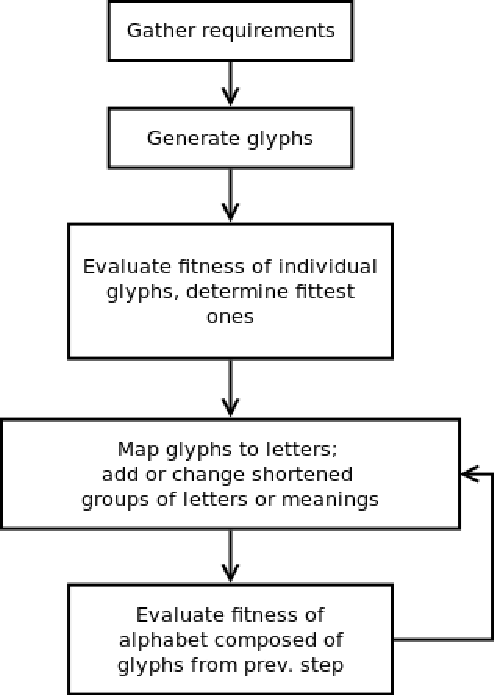
\includegraphics[width=0.75\hsize]{f.pdf}
\caption{Basic description of framework.}
\end{figure}

As this is a framework for the creation of alphabets in general, the goal is not to give any final recommendations about concrete alphabets, they should be formulated individually for each alphabet. However, the following requirements are used as base in this paper, and should generalize well for almost any alphabet, independently of the medium, dimensionality and purpose:
\begin{itemize}
        \item The individual glyphs should be as easy to write as possible, as long as it's still possible to differentiate them. (Oversimplified glyphs degenerate into straight lines, which is counterproductive).
        \item The glyphs most likely to be together should be likely to connect easily.
        \item The more simple glyphs should be mapped to the most common symbols.
        \item If certain glyphs are often found together, the possibility of replacing them with one glyph should be evaluated.
\end{itemize}

\section{Gathering requirements for the needed alphabet}

As mentioned in the Introduction, most writing systems have been heavily influenced by the constraints inherent in their area of use --- purpose, characteristics of the information they needed to convey, materials used. When synthetic systems of symbols are created or generated, they similarly are constrained, but can't be polished by millennia of continuous use. And lastly, even if there were millennia to let those systems evolve, even naturally evolving systems tend to converge towards local optima rather than a global optimum (as is the case with genetic algorithms). Requirements and use patterns may gradually change, while the systems may be stuck in a state that is not optimal anymore, being unable to sacrifice short-term fitness for long-term fitness. (This might be considered an example of path dependence.) Therefore, before attempting to create a system from zero, a very careful analysis of the requirements and limitations is needed.

For our example of creating a shorthand system (trivial use case), the following may be considered:
\begin{enumerate}
        \item On a purely symbolic level:
        \begin{enumerate}
                \item Writing letters
                \begin{enumerate}
                        \item number of strokes needed to encode individual letters
                        \item complexity of the resulting glyph
                \end{enumerate}
                \item Writing words
                \begin{enumerate}
                        \item connections between individual letters (glyphs)
                        \item how likely are letters that are easy to connect to each to be represented by easily connectable glyphs
                        \item if all existing glyphs are not identical in complexity, what is the ratio of easy-to-write glyphs to the complex ones in a typical text (the bigger the ratio, the better)
                \end{enumerate}
        \end{enumerate}
        \item Writing sentences:
        \begin{enumerate}
                \item are there any often-repeating words or groups of words which, when replaced by a shorter, even if complex, symbol, would lead to a gain in time? ("The" as a typical example).
        \end{enumerate}
        \item On a semantic level: Are there any grammatical categories or modalities that are represented in natural text with many letters, that when replaced by a single glyph or a modifier, would lead to a gain in time? (tenses, number, gender, hypotheticals, ...). For example, in our manually generated shorthand system, time, modality, and person were encoded via a single glyph consisting of three parts, which allowed to considerably shorten groups like "they would have been able to".
        \item On an information theoretical level: How much redundancy is needed? How many errors in transcription can happen before the message becomes either unreadable or its meaning is distorted?  (Natural languages  are redundant via multiple mechanisms, notably via agreement in person, gender, case...~\citep{bussmann2006routledge} Errors or interferences will still allow to understand what’s being said, up to a certain point. This may not be the case for constructed writing systems, if they are built with low redundancy)~\citep{reza1961introduction}.
\end{enumerate}

There may be different ways to quantify the above. One way would be analyzing source texts written by the person (or representative sample of people) who will be using the system, to fit it to their speech patterns and word use. At the end, the following basic information should be available:

\begin{itemize}
        \item frequencies of individual letters \(p_i\)
        \item most-needed connections \(c_{ij}\)
\end{itemize}

As example of how the information can be used, let's consider again our hypothetical shorthand system. Each of the generated glyphs can have three possible starting and ending strokes, represented by integers, and positioned at different heights.\(I_s, I_e=\{0, 1, 2\}\) Glyphs \(i, j\) where \(i_e=j_s\) are considered easily connectable. Using this information, later we can map the glyphs to meanings in such a way, that the letters that are most likely to follow each other are more likely to be
represented by easily connectable glyphs. The problem would be trivially solvable by having all glyphs start and end at the same point, but this would make it harder to differentiate the individual glyphs.

\section{Generation of the glyphs}
The second part of the proposed framework is the generation of possible glyphs. In this paper, Bezier curves have been used to generate the glyphs and calculate some of the needed metrics.
During the generation of the example glyphs, we made the following assumptions about the alphabet for which the glyphs are generated:
\begin{enumerate}
        \item The glyphs have a definite starting and ending point; the number of such points is limited, to facilitate connecting the symbols to each other.
        \item The stroke width does not vary (as, for example, in the case of Pitman shorthand), because of the low availability of pens able to convey even two levels of thickness and of low average penmanship skill in most people. (Though using it as a third or fourth dimension would certainly be possible.)
        \item The symbols will fit into a square bounding box.
\end{enumerate}
For each letter, multiple glyphs are generated. The generation of glyphs starts by fixing a definite starting and ending point and then adding a semi-random number of control points. The number of control points used in the generation of the specific glyph is selected via a normal distribution, with the average number being the mean of the distribution and with standard deviation being calculated based on the maximum number of control points. While one of the criteria for the glyphs is their
simplicity, extremely simple symbols are counterproductive, and we needed to prevent the alphabet from degenerating to straight and diagonal lines. Additionally, variation in the gene pool is crucial in genetic algorithms, if one is to be used later on. Therefore, a degree of randomness in all phases is needed, and this is one way to provide it. Figures 2-5 are examples of glyphs generated using the above rules.

\begin{figure}[tbp]
\centering
        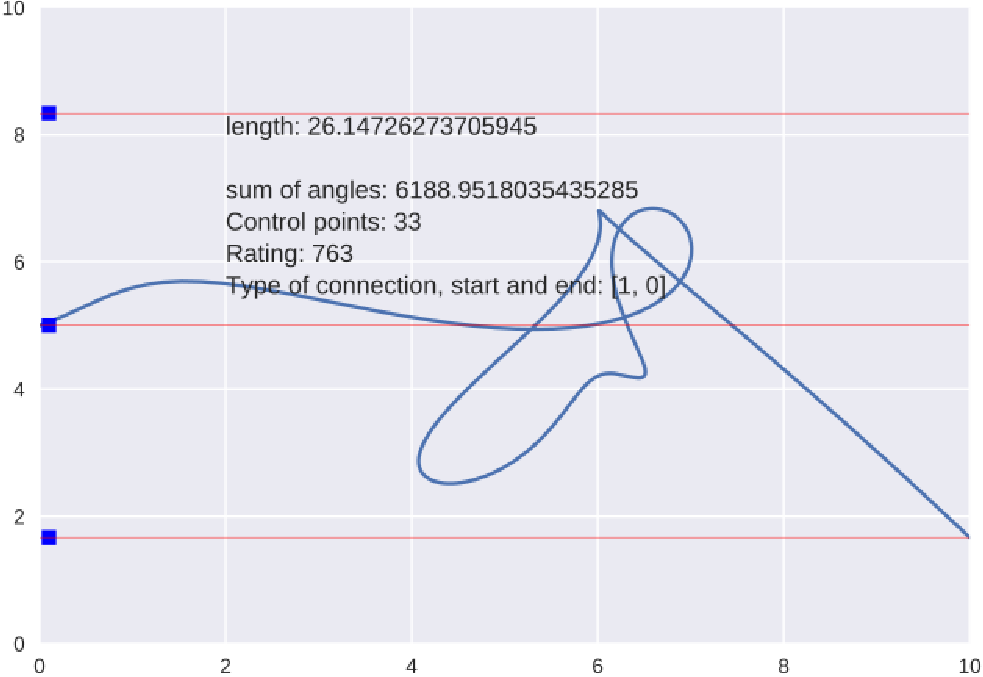
\includegraphics[width=0.75\hsize]{e1.pdf}
\caption{Example of generated glyph with low fitness}
\end{figure}
\begin{figure}[tbp]
\centering
        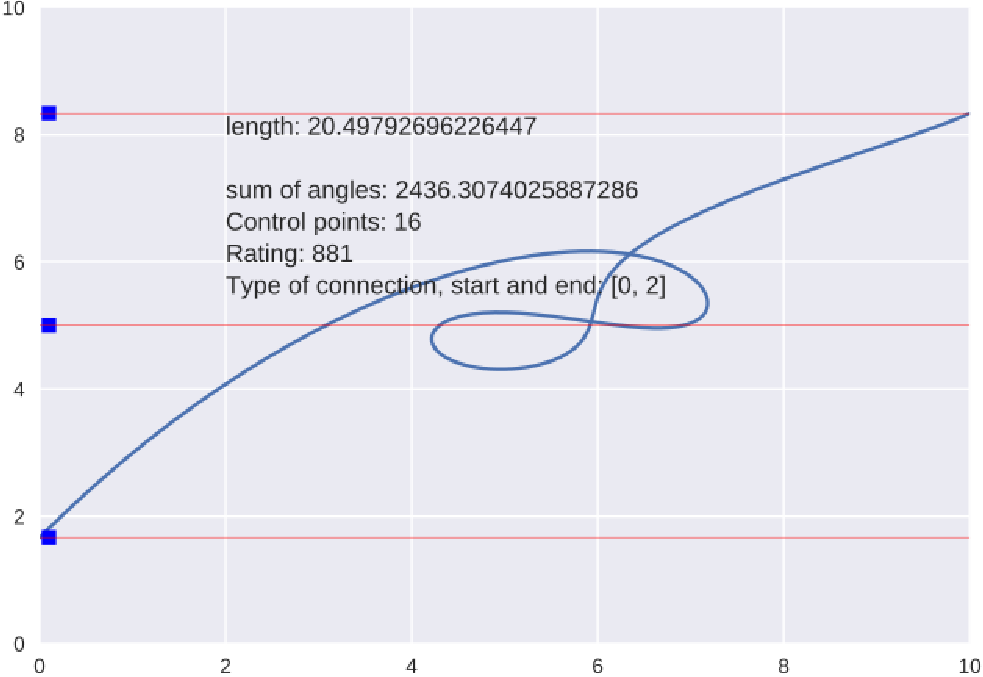
\includegraphics[width=0.75\hsize]{e3.pdf}
\caption{Glyph with higher fitness      }
\end{figure}
\begin{figure}[tbp]
\centering
        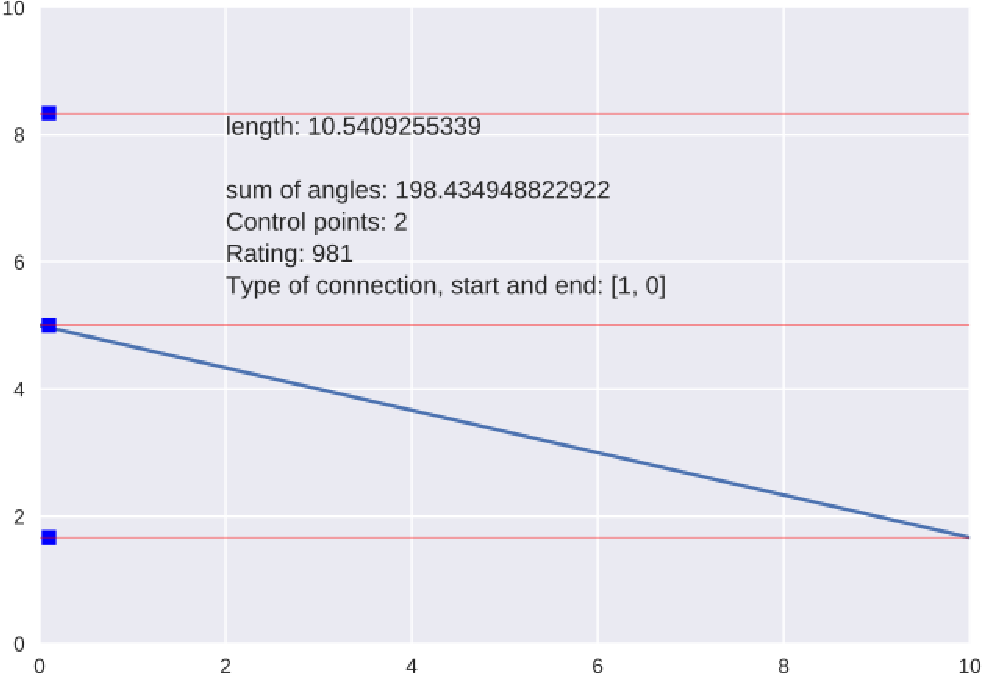
\includegraphics[width=0.75\hsize]{e4.pdf}
\caption{Too many extremely simple symbols would not be desirable}
\end{figure}
\begin{figure}[tbp]
\centering
        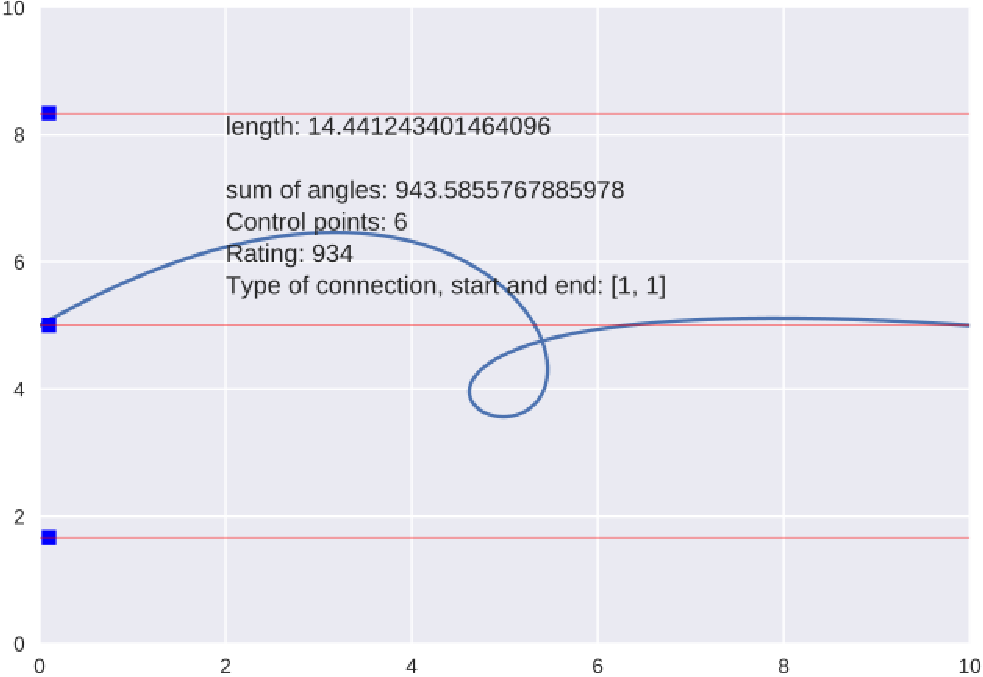
\includegraphics[width=0.75\hsize]{e2.pdf}
\caption{The simpler a glyph is, the higher fitness it has}
\end{figure}

\balance

\section{Evaluating the fitness of the individual glyphs}
In this stage, the fitness of each glyph is determined. Many approaches are possible, and they heavily depend on the context and the medium for which the generation is being done. For our shorthand system, the main criteria were length and simplicity. The number of control points has been used as a proxy of fitness and has been partly accounted for in the generation phase (empirically, the more control points the more chaotic the glyph is). The second metric is complexity, which may be loosely
defined as “how hard it would be to write this symbol using a pen”. For our purposes, complexity is defined as \(\frac{c}{l}\), where \(c\) is the sum of the angles in the polygonal representation of the curve (informally, how curved the glyph is; the more curves there are and the sharper the individual curves are, the bigger the value is), and \(l\) is the length of the curve (a certain amount of curves on a large glyph should not be penalized as much as the same amount on a smaller one). C is calculated by converting the curve between the first adjoining control points to a polygon, summing the absolute value of the angles between all adjoining lines, and repeating the process for all the successive control points.
\(c=\sum_{i=1}^n\sum_{j=2}^{p}L_n(j_i, j_i-1)\), where \(n\) is the number of control points,  \(p\) is the number of lines used to approximate the curve, L is the angle between two lines,  and \(j_i\) is the line after the control point \(i\). 

The reasons for defining \(c\) as we did are manifold, one of them being that a very similar metric is used for evaluating the similarity of the two glyphs to each other. Much better metrics are possible.

Generally, quantifying fitness of a particular glyph might make use of quite a lot of variables, for example:
\begin{itemize}
        \item number (percentage?) of strokes which are known to be easy or hard to write (writing a stroke from upper-left to bottom-right might be harder for some people, for example, due to the right slant in their handwriting). 
        \item how easy is a stroke to remember. This might not map perfectly to simplicity, due, for example, to characteristics of human memory like the Von Restorff effect~\citep{hunt1995subtlety}
\end{itemize}
	The subjective reactions to signs might vary between people, differences due to age, cultural and/or language background are probable. This might be a promising area to study with the help of machine learning. Data like "Symbols similar to X perform poorly with demographic Y" would be valuable for creating alphabets when something about the probable users is known (which alphabet or writing system is more familiar to them? How much new information are they probably able to learn and for how much they are able to retain it? Did they learn thousands of hieroglyphics since they were children? How motivated are they?). 

Additionally, machine learning would open the doors for custom-tailored systems, where users rate some symbols and based on their feedback predictions are made about what other symbols they might like, remember and use. And, as mentioned previously, their particular use patterns might dictate different mappings of symbols to meanings (letters, actions, preferences). 
\section{Mapping symbols to meanings}
The first mapping of the generated glyphs, before its fitness is rated, is necessarily very tentative. At the beginning, we suggest just mapping the letters to glyphs by ordering the glyphs in decreasing order of fitness and pairing them with letters, ordered by their frequency. This would give a good starting point, which can be further improved in the next step by taking into account how easy the letters are to connect and the other requirements. 

In this paper we have not touched grammatical modalities and ways to shorten them in great detail, as they would merit quite a lot more research and space (and, probably, their own paper); regardless, they would have their place at this step of the framework. 
\section{Evaluating the fitness of an alphabet}
For an alphabet, our goals could be the following:
\begin{enumerate}
        \item As much high-fitness letters as possible
        \item Letters which are found the most often should have the highest fitness (that is, be as simple as possible).
        \item The letters should be unlike to each other
\end{enumerate}

The most important requirement is for the letters to be unlike each other. This is needed both for the resulting text to be readable (the existance of a 1-to-1 mapping between a text written in shorthand and a normal text, or at least for the resulting text being readable using contextual clues) and for improving the memorization of the glyphs (memorizing many similar stimuli is much harder than many different ones, unless a good framework for memorization is given, such as dividing symbols in parts). 

For our purposes histogram comparison was the most straight-forward to implement. The data for the histogram is provided by the angles computed at the previous step. Basic shapes and turns would be recognizable, and the difference between the two makeshift histograms would approximate the difference between the glyphs. Here, \(D_{ij}\) is the difference between glyphs \(i, j\).

Therefore, one formula for the fitness could be:
\[
f=\sum^{n}_{i=1}f_i+
\sum^{n}_{i=1}\sum^{n}_{i=1}D_{ij}+
\sum^{n}_{i=1}f_ip_i
\]
and the glyphs are picked so that the above formula is maximized. (The formula above does not include connections.)

A genetic algorithm at this point would attempt adding/removing/moving control points, switching glyphs between letters, introducing mirror-distortions etc. etc.

\section{Discussion and future work}
The basic ideas of this framework can be applied for the generation of any alphabet used in the real world. For touchpads, for example, connections may be built not using three possible endings, but 2D-points on the screen instead, and multitouch and weight-sensitivity may be included in the generation. By adding dimensions, 3D-gestures alphabets may be created. Much better heuristics for fitness may be created by more precise algorithms, machine learning and use of biology and cognitive science. The approaches demonstrated here are general enough to allow an enormous amount of flexibility in the kind of alphabets they may be used to create.
	One of the more interesting avenues of further research would be creating algorithms for mapping glyphs to semantics, both to letters and to more complex grammar categories or structures. Finding (with AI?) the categories which could be shortened to one or two symbols is challenging by itself, but not all of the possible patterns found by an AI would be intuitive enough for a person to use or even to understand. 

\bibliographystyle{myIEEEtran}
\bibliography{mybib}


\end{document}

